\documentclass[ ngerman, fontsize= 12pt, paper=a4, headings=big, titlepage=true]{article}

%Sprache
\usepackage{babel}
\usepackage[utf8]{inputenc}
\usepackage[T1]{fontenc}
\usepackage{mathptmx}
\usepackage{hyperref}
\usepackage{lmodern, microtype}
\usepackage{csquotes}
\usepackage{hyperref}
\usepackage{enumerate}

%\usepackage[onehalfspace]{setspace}
%Tablellen:
\usepackage{multirow}
\usepackage{caption}
\usepackage{booktabs}
\usepackage{rotating}
\usepackage{hhline,float}
%\usepackage{pdfpages}

%Mathematik
\usepackage{amsmath}
\usepackage{amsfonts}
\usepackage{amssymb}
\usepackage{mathtools}
\usepackage{bbm}

%Grafik
\usepackage{wrapfig}
\usepackage{color}
\usepackage[svgnames]{xcolor}
\usepackage[
left=3cm,
right=2cm,
top=2.5cm,
bottom=2cm,
%includeheadfoot
]{geometry}

%R-Code
\usepackage{listings}
\lstset{language=R,
	basicstyle=\small\ttfamily,
	stringstyle=\color{DarkGreen},
	otherkeywords={0,1,2,3,4,5,6,7,8,9},
	morekeywords={TRUE,FALSE},
	deletekeywords={data,frame,length,as,character},
	keywordstyle=\color{blue},
	commentstyle=\color{DarkGreen},
}

\begin{document}
	
	
\begin{center}
	\Large
	Technische Universität Dortmund\\
	Fakultät Statistik\\
	Sommersemester 2021\\
	
	\vspace{4em}
	
	Grundlagen der Versuchaplanung: Bericht über das 2.Experiment
	
	\Huge
	\textbf{Temperaturexperiment}
	
	\Large
	\vspace{5em}
	Dozenten:\\
	JProf. Dr. Kirsten Schorning, M.Sc. Onur Gül, B.Sc. Wiebke Dammann\\
	
	
	\vspace{8em}
	Autorinnen: \\
	Kaya Maria Bayer\\
	Ketevan Gurtskaia\\
    Danuscha Große-Hering\\	
	Alicia Hemmersbach\\

	
	
	\vspace{12em}
	
	05.Juli 2021
	
\end{center}

\newpage	

\tableofcontents
\newpage

\section{Einleitung}
Ein Thermometer besitzen vermutlich die meisten Haushalte. Einige davon besitzen wahrscheinlich auch ein Thermometer, welches die Temperatur draußen und drinnen messen kann. Möglicherweise hat man sich bereits die Frage gestellt, worin der Unterschied zwischen dem Innen- und Außensensor dieser Thermometer liegt und ob dieser lediglich darin besteht, dass Außensensoren wetterfest sind, oder ob beide Sensoren, unabhängig von weiteren äußeren Einflüssen, die gleichen Temperaturen messen würden, wenn man den Innensensor nach außen und den Außensensor nach innen legt. \newline 
Genau dieser Frage wird in dem folgenden Temperaturexperiment nachgegangen. Es soll überprüft werden, ob es Unterschiede bei den Messungen der beiden Sensoren drinnen und draußen gibt. \newline
Dazu sollen mit 10 gleichen Thermometern einige Messungen drinnen und draußen durchgeführt werden. Hierbei wird dann der Unterschied der zwei gemessenen Temperaturen zwischen Innen- und Außensensor ausgewertet und mit Hilfe eines statistischen Tests interpretiert. \newline 
Im Folgenden wird auf die Problemstellung des Experiments und die Versuchsbedingungen, dann auf die Analyse des Problems, das zugehörige statistische Modell, die Hypothesen, die statistischen Auswertungsmethoden des Experiment und die Versuchsplanung eingegangen.
\section{Problemstellung und Versuchsbedingungen}
Ziel des Experimentes ist es, herauszufinden, ob die Messungen der Innen- und Außensensoren am selben Ort bei gleicher Temperatur übereinstimmen, oder ob es Unterschiede gibt. Außerdem soll untersucht werden, ob es einen Unterschied macht, ob draußen oder drinnen gemessen wird.\newline
Um diese beiden Fragestellungen zu beantworten, sollen insgesamt 6 Messungen mit jeweils 10 Thermometern, die einen Außen- und einen Innensensor haben, durchgeführt werden, sodass nach der Durchführung des Experimentes 120 Messwerte vorliegen. Dabei sollen alle Thermometer gleich alt und zudem möglichst neu sein. Außerdem dürfen die Thermometer keine sichtbaren oder bekannten Schäden haben. Die Messungen werden in 2 Zeitslots über einen Tag verteilt, an dem keine extremen Wetterbedingungen herrschen, vorgenommen. Somit wird sichergestellt, dass in beiden Zeitslots ähnliche Temperaturen vorliegen. Außerdem werden die Thermometer vor jeder Messung randomisiert in 2 Gruppen mit jeweils 5 Thermometern aufgeteilt. Die eine Gruppe der Thermometer misst die Temperatur draußen und die andere Gruppe der Thermometer misst die Temperatur drinnen. Der Raum, in welchen die Innenmessungen stattfinden, soll hierbei keine angeschaltete Heizung oder Klimaanlage haben. Außerdem sollen, falls vorhanden, alle Fenster geschlossen und soweit abgedunkelt sein, dass keine direkte Sonneneinstrahlung, zum Beispiel durch Fenster, auf die Thermometer trifft. \newline
Die Messungen draußen sollen an einem windgeschützten Ort ohne direkte und auch ohne gespiegelte Sonneneinstrahlung, zum Beisiel durch Wasser, stattfinden. Außerdem sollten die Thermometer an einem trockenen Ort platziert werden und es sollten andere direkte Wärmequellen mindestens 10 Meter Abstand von dem Messort haben. \newline
Für die Messungen werden die 5 Thermometer draußen und die 5 Thermometer drinnen jeweils nebeneinander auf einen ebenen identischen Tisch gelegt. Außerdem ist darauf zu achten, dass die Innen- und Außensensoren direkt nebeneinander liegen.  \newline
Es werden jeweils 3 Messungen pro Thermometer in 2 Zeitslots durchgeführt. Der erste Slot ist von 4:00 - 6:00 Uhr und der zweite Slot von 16:00 - 18:00 Uhr. Insgesamt beträgt jeder Zeitslot zwei Stunden. Zu Beginn der Zeitslots werden die Thermometer für 15 Minuten in den Kühlschrank gelegt. Somit wird die Temperatur von allen Thermometern gleichmäßig neutralisiert. Nach Ablauf der 15 Minuten werden die Thermometer dann von 2 Versuchsleitern aus dem Kühlschrank entnommen und auf dem dafür vorgesehenen Tisch platziert. Dabei ist ein Versuchsleiter für die Thermometer draußen und ein Versuchsleiter für die Thermometer drinnen zuständig. Die Thermometer sollen jeweils 20 Minuten auf dem Tisch liegen und sich der jeweiligen Temperatur anpassen, bevor die angezeigten Temperaturen von den anderen beiden Versuchsleitern abgelesen und notiert werden. Nach der ersten Messung in beiden Slots kommen alle Thermometer für 15 Minuten zurück in den Kühlschrank, damit sich die Temperatur erneut neutralisieren kann. Nach Ablauf der 15 Minuten werden die Thermometer wieder von den ersten beiden Versuchsleitern auf dem Tisch platziert. Darauf hin werden die Temperaturen 20 Minuten abgelesen und notiert. Die dritte Messung in beiden Zeitslots läuft nach dem gleichen Schema so ab. Es ist zu beachten, dass das Ablesen und Notieren der Werte möglichst schnell passiert, damit alle 5 Werte jeweils zur gleichen tatsächlich herrschenden Temperatur abgelesen werden. In der möglicherweise verbleibenden Zeit der Slots und zwischen dem ersten und zweiten Slots können die Thermometer jeweils auf den Tischen liegen bleiben, wobei auch hierbei darauf zu achten ist, dass sie in der Zwischenzeit keinem Regen oder anderen Wetterextrema ausgesetzt sind.



\section{Analyse des Problems}

%was ist die interessiernde abhängige Variable?
Es soll untersucht werden, ob die Messungen der Innen-und Außensensoren der Thermometer gleich sind, ist die vorliegende interessierende Variable die Temperaturdifferenz der Innen-und Außensensoren:\\
\begin{center}
	%$y_{\text{Differenz}} = y_{\text{Außensensor}}-y_{\text{Innensensor}} $
	$y_{\text{\tiny{Differenz}}} = y_{\text{\tiny{Außensensor}}}-y_{\text{\tiny{Innensensor}}} $
\end{center}

%Was ist die interessierende Einflussvariable udn wie können diese variiert werden?
Die wahre Temperatur ist eine Einflussvariable. Diese können wir jedoch nicht kontrollieren.  Zudem ist auch der Ort des Thermometers eine interessierende Einflussvariable, welche wir kontrollieren können. In dem Versuch werden wir zwei feste Orte festlegen: Innerhalb und Außerhalb eines Gebäudes. \\

%Was sind mögliche Störvariablen und welche können kontrolliert werden?

Im folgenden werden mögliche Störvariablen genannt und inwiefern man diese kontrollieren kann. Generell haben die Wetter-bzw. die Klimabedingungen einen hohen Einfluss auf den Versuch.  In geschlossenen Räumen ist dies die Nutzung einer Heizung oder Klimaanlage und die Luftfeuchtigkeit. Die Klimabedingungen im Raum werden Konstant gehalten. Das bedeutet, dass sowohl die Klimaanlage, wie auch die Heizung oder Anlagen zur Regulierung der Luftfeuchtigkeit, ausgeschaltet werden. Außerhalb eines Gebäudes fällt auch die Luftfeuchtigkeit, die Sonnenbestrahlung an dem Messort, die Windstärke, wie auch Regen. Auch diese Bedingungen möchten wir möglichst konstant halten. Dies wird umgesetzt, indem die Thermometer an windgeschützten und überdachten ohne direkter Sonnenbestrahlung platziert werden sollen. Neben diesen Wetterfaktoren, kann auch das Thermometer einen Einfluss haben. Zum einen können Messungenauigkeiten zwischen unterschiedlichen Gererätehersteller oder Modellen zusätzlich zu den Messungenauigkeiten der einzelnen Thermometer dazukommen. Dies würde dazu führen, dass unser Versuch komplizierter würde. Deswegen halten wir das Modell des Thermometers konstant. Zudem ist die Tageszeit bzgl. der unterschiedlichen Temperaturen am Tage eine Störvariable. \\

%Von welchen Störvariablen soll noch der Einfluss erfasst werden?
Zusammengefasst sollen die meisten Störvariablen möglichst konstant gehalten werden und somit soll dessen Einfluss nicht erfasst werden. Jedoch können wir sie Messzeiten beeinflussen.  \\

%Welche Störvariablen sollen als Blockvariablen aufgefasst werden?
Durch die Variation der Messzeiten ist eine Variation der Temperatur möglich. Das bedeutet genauer: Zur Zeit des Sonnenaufgangs ist es tendenziell kälter, als zur Nachmittagszeit.\cite{WK2}. Deswegen wird die Messzeit als Blockvariable mit zwei Stufen aufgefasst. Dabei  entspricht die erste Stufe die Morgenstunden und die zweite Stufe die Nachmittagsstunden. 



\section{Modell, Hypothesen und statistische Auswertungsmethoden}
\section{Versuchsplanung}

\newpage
\section{Versuchsablauf}
Zunächst muss bestimmt werden, welche Personen Innen/Außen die Thermometer aufstellen und die Messungen ablesen und dokumentieren. \ref{Verteilung}
\begin{table}[h]
	\begin{tabular}{l|l|l}
		
		Uhrzeit		&	Beschreibung									&	Versuchsleiterin \\
		\hline
		03:30 Uhr	&	Vorbereitung der Messorte						& alle\\
		03:55 Uhr	&	Aufstellen der Thermometer						& D.Grosse-Hering/K.Bayer\\
		04:00 Uhr	&	Beginn der 1.Messung							& \\
		04:20 Uhr	& 	Ende der 1.Messung: dokumentieren, Zwischenlagerung & A.Hemmersbach/K.Gurtskaia\\
		
		04:40 Uhr	&	Aufstellen der Thermometer						&D.Grosse-Hering/K.Bayer\\
		04:45 Uhr	&	Beginn der 2.Messung							& \\
		05:05 Uhr	& 	Ende der 2.Messung: dokumentieren, Zwischenlagerung & A.Hemmersbach/K.Gurtskaia\\
		
		05:25 Uhr	&	Aufstellen der Thermometer						&D.Grosse-Hering/K.Bayer\\
		05:40 Uhr	&	Beginn der 3.Messung							& \\
		06:00 Uhr	& 	Ende der 3.Messung: dokumentieren, Zwischenlagerung & A.Hemmersbach/K.Gurtskaia\\
		
		\hline
		06:20 Uhr	& 	Pause											& alle \\
		\hline
		
		15:55 Uhr	&	Aufstellen der Thermometer						&A.Hemmersbach/D.Grosse-Hering\\
		16:00 Uhr	&	Beginn der 1.Messung							& \\
		16:20 Uhr	& 	Ende der 1.Messung: dokumentieren, Zwischenlagerung &K.Bayer/K.Gurtskaia \\
		
		16:40 Uhr	&	Aufstellen der Thermometer						&A.Hemmersbach/D.Grosse-Hering\\
		16:45 Uhr	&	Beginn der 2.Messung							&K.Bayer/K.Gurtskaia\\
		17:05 Uhr	& 	Ende der 2.Messung: dokumentieren, Zwischenlagerung &\\
		
		17:25 Uhr	&	Aufstellen der Thermometer						&A.Hemmersbach/D.Grosse-Hering\\
		17:40 Uhr	&	Beginn der 3.Messung							& \\
		18:00 Uhr	& 	Ende der 3.Messung: dokumentieren, Zwischenlagerung & K.Bayer/K.Gurtskaia\\
		
		\hline
		
		18:20 Uhr	&	Nachbesprechung									& alle \\
		18:50 Uhr	& 	Digitalisierung der Messdaten					&\\
		
		
	\end{tabular}
\end{table}
\newpage
\textcolor{white}{\section{Literatur}}
\bibliography{Literatur} 
\bibliographystyle{alphadin}
 
 \newpage

\renewcommand{\thesubsection}{\Alph{subsection}}


\section{Anhang}

\subsection{Aufgaben Verteilung} \label{Verteilung}
\begin{lstlisting}
	Versuchsleiterin <- c("K.Bayer","A.Hemmersbach","D.Grosse-Hering","K.Gurtskaia")
	
	set.seed(1539)
	
	#Morgens Innen
	sample(Versuchsleiterin,2)
	## "D.Grosse-Hering" "A.Hemmersbach" 
	
	#Morgens Aussen
	##"K.Bayer" "K.Gurtskaia"
	
	set.seed(1540)
	
	#Nachmittags Innen
	sample(Versuchsleiterin,2)
	##"A.Hemmersbach" "K.Bayer"
	
	#Nachmittags Aussen
	## "D.Grosse-Hering" "K.Gurtskaia"
	
	set.seed(1540)
	#Digitalisierung der Daten
	sample(Versuchsleiterin,1)
	##"A.Hemmersbach"
\end{lstlisting}

Die Erstgenannte Person wird für die Aufstellung der Thermometer und die zweitgenannte Person ist für die Dokumentierung der Messdaten zuständig.	

\begin{figure}[t]
	\subsection{Erklärung zum Bericht}
	\hspace{-2.3cm}
	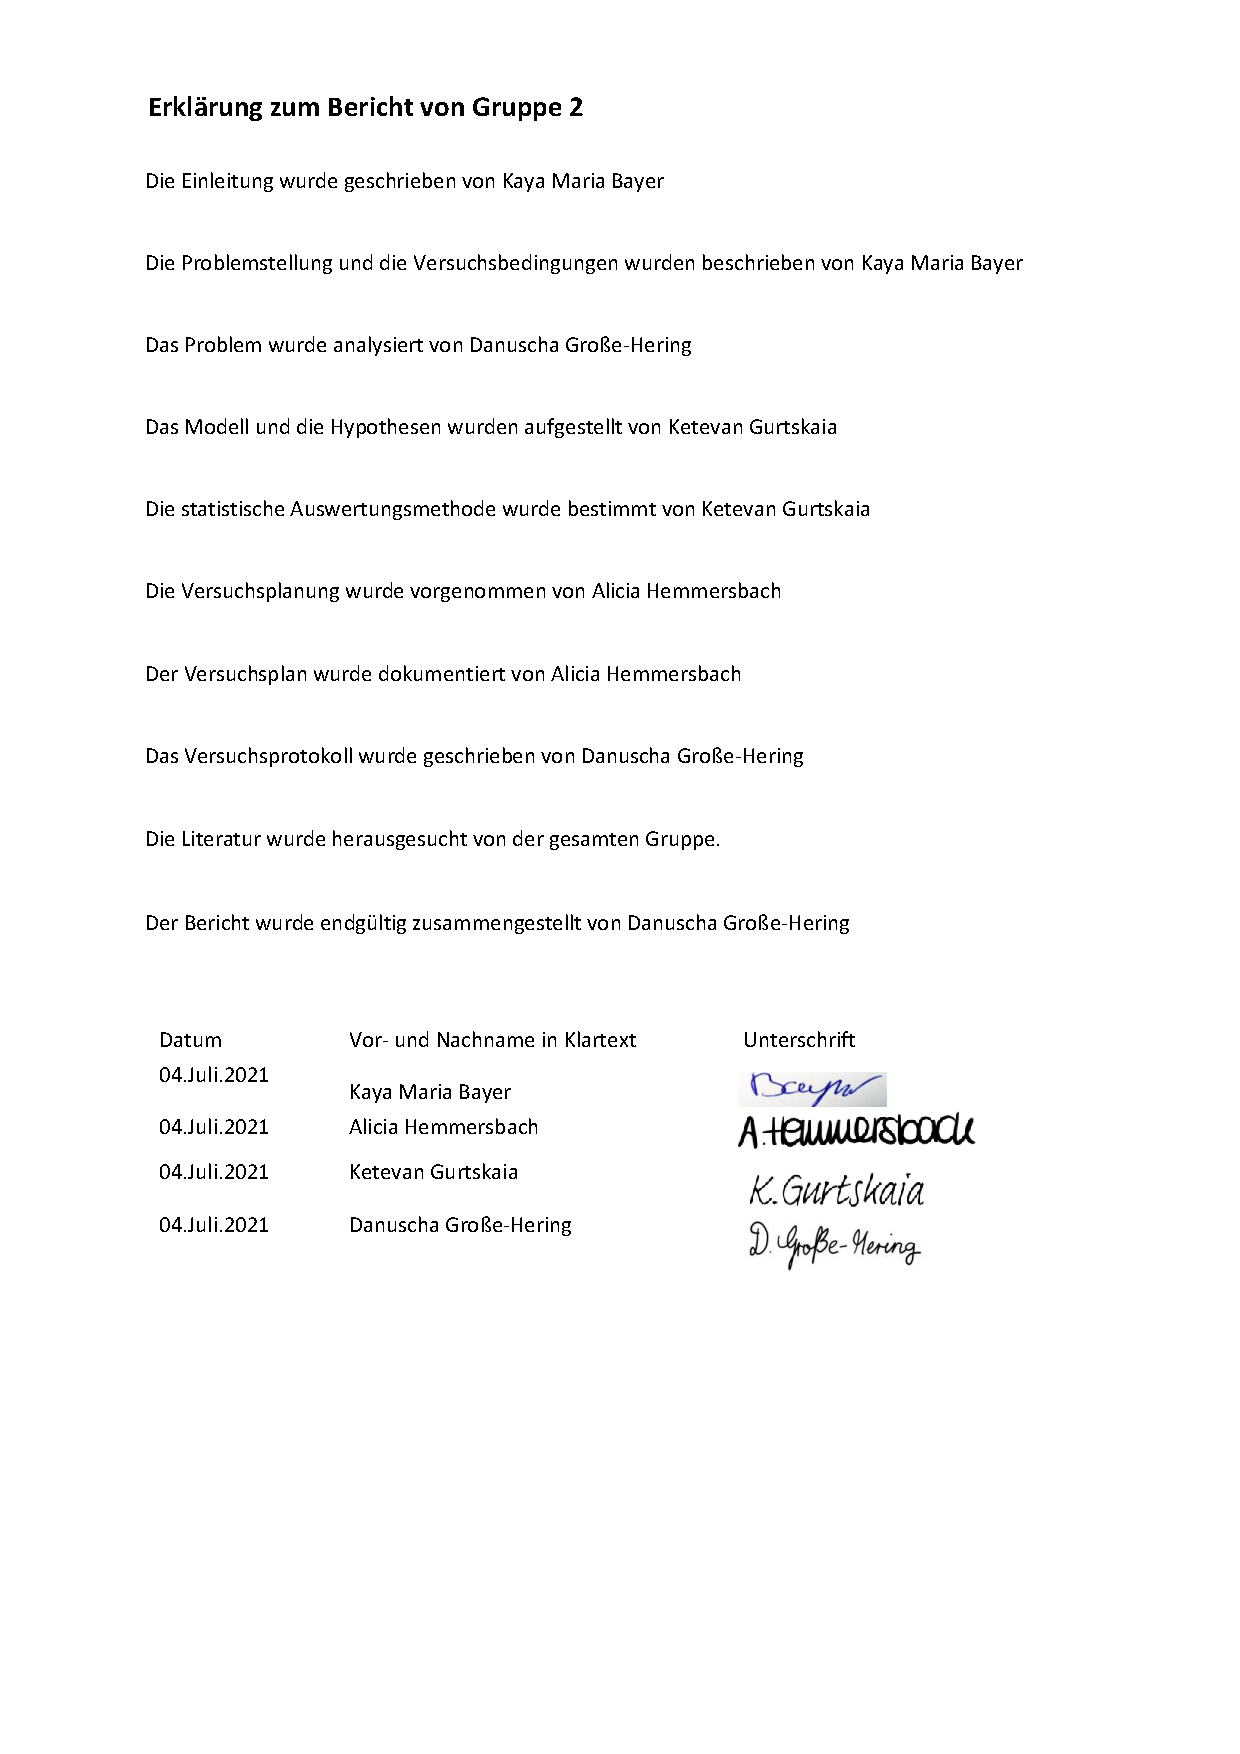
\includegraphics[scale=0.8]{ErklaerungzumBericht}
\end{figure}


\end{document}


